\chapter{Primera Iteración: Prototipo inicial}

\section{Arquitectura del Proyecto}
\label{it1arquitectura}
La arquitectura del proyecto está caracterizada por la dinamicidad y capacidad para adaptarse de sus clases. Permitiendo que tomen un rol u otro dependiendo de las clases que las definan. Es decir, una clase personaje debe adaptarse al rol de personaje que le toque interpretar, y al contexto que le pone dentro de la escena. Además, debe seleccionar el recurso que lo represente que cumpla con las condiciones que se den en ese momento dentro de la escena. Finalmente debe permitir la interactuación y ejecución de efectos que están asignados a si mismo.

En esencial, esto se puede explicar con el diagrama de clases muy simplificado de la figura 3. Este diagrama fue generado en esta iteración del proyecto, por lo que su formato es muy diferente al resto de diagramas que se muestran en posteriores iteraciones.

\begin{figure}[htb]
	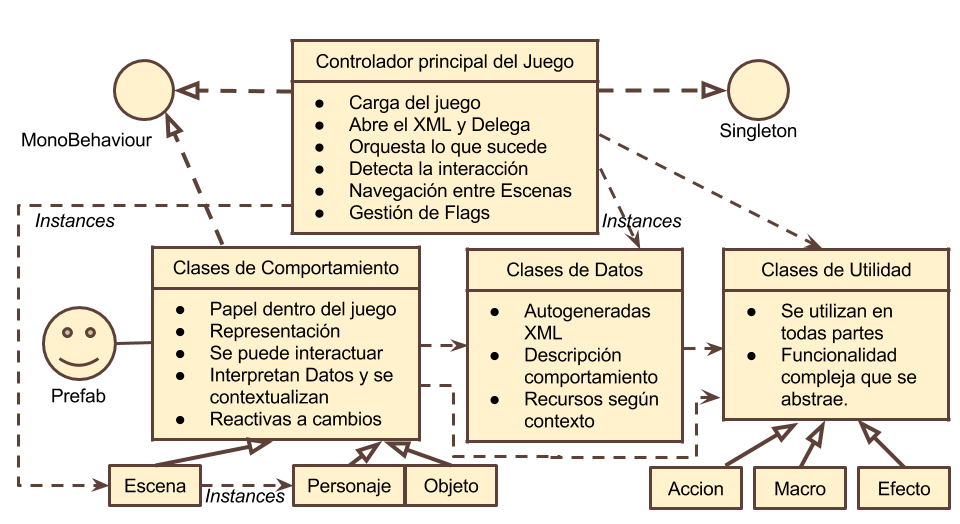
\includegraphics[height=3.5in]{figures/arquitecturait1.png}
	\caption[Arquitectura simplificada - Prototipo 1]{Diagrama de clases simplificado de la arquitectura de clases de la primera iteración del proyecto.}
	\label{arquitecturait1}
\end{figure}

En la figura \ref{arquitecturait1} hay varios elementos que no son comunes en un diagrama de clases. El primero de ellos es la "Cara sonriente" que aparece a la izquierda con el texto \textit{Prefab} debajo de el. Este \textit{Prefab} es un elemento en Unity3D que resume el concepto de Objeto Prefabricado, y que, contiene, una representación tridimensional, junto a todas las componentes y comportamientos que definen dicho objeto. Por otra parte la interfaz \textit{MonoBehabiour} no es una interfaz, sino una clase abstracta, y esta, provee a los elementos que la extienden de la habilidad de ser componentes para los objetos de la escena. Dicha clase contiene varios métodos como Start(), Awake() o Update() que permiten a estos comportamientos inicializarse, actuar, y en esencia, tener una fracción de tiempo para realizar acciones dentro de la escena de Unity3D.

En la figura \ref{arquitecturait1} encontramos cuatro tipos de clases:

\begin{itemize}
	\item El controlador principal del juego.
	\item Las Clases de Datos
	\item Las Clases de Comportamiento: Escenas, Personajes, Objetos, Salidas, etc...
	\item Las Clases de Utilidad: Acciones, Efectos, Macros, Secuencias, Diálogos, etc...
\end{itemize}

Todas las clases que se presentan en este primer prototipo han sufrido cambios muy grandes o totales tanto en su código, como en su funcionalidad. Algunas de ellas han desaparecido, surgiendo clases nuevas que realizan su funcionalidad, otras se han transformado completamente o han sido asumidas por otras, y finalmente, otras han surgido de la generalización y refactorización de código.

\subsection{Controlador Principal de Juego}

El controlador principal de juego, implementado con una clase de nombre Game, se encarga de, en primer lugar, comenzar la carga del juego, comenzando a explorar el XML y delegando en las Clases de Datos su propia interpretación, así como orquestar lo que sucede dentro del juego, detecta la interacción por parte del jugador y notifica a aquellos elementos cuando se interactúa con ellos, realiza la navegación entre escenas cuando es necesario, y controla el estado de los interruptores que controlan las condiciones para la contextualización de cada escena en su momento apropiado.


Implementa el patrón Singleton, pues sólo una instancia es necesaria para el control.

\subsection{Clases de Datos}

Las clases de datos se encargan de generarse a partir de un elemento del fichero XML y sirven de descripción para una Clase de Comportamiento para representarse y interactuar de la forma correcta en cada momento. A través del documento XML realizan una lectura del mismo mediante la librería de c\# System.Xml, y rellenan sus atributos a partir de la especificación en dicho XML. Asimismo implementan funciones útiles como la obtención de un paquete de recursos apropiado según el contexto.

Existe una clase de datos por cada Clase de Comportamiento, aunque también existen clases de datos auxiliares mucho más pequeñas y que apenas aportan funcionalidad, siento meros contenedores de datos.

\subsection{Clases de Comportamiento}

Las clases de comportamiento son aquellas clases que juegan un papel dentro del videojuego y participan de forma activa en la representación del mismo. Dentro de esta categoría encontramos a las Escenas, los Personajes, los Objetos, las Salidas de las escenas, así como los objetos de atrezo y todos aquellos elementos que tienen una representación virtual en el videojuego. 

Cada una de estas clases heredará de la clase de Unity \textit{MonoBehabiour}, que indica, como se explica en la sección \ref{it1arquitectura}, que dicha clase es un comportamiento y se puede asignar como componente a un elemento de la escena. Cada una de ellas tiene un objeto de datos que debe interpretar. Esta clase de comportamiento recibirá estímulos por parte del controlador principal del juego cuando el jugador interactue con ellas. Este paso intermedio es necesario ya que hay momentos en los que el controlado principal debe evitar la interacción del jugador con dichos elementos por encontrarse en mitad de un diálogo. Con este estímulo, la clase de comportamiento gestiona las diferentes interacciones que tenga el usuario con si mismo.

Finalmente, estas clases se encapsulan dentro de un \textit{Prefab}, formando parte como componente de un objeto tridimensional, junto a otras componentes.

\section{Detalles de la implementación}

Existen algunas cuestiones cruciales y generales acerca de cómo se realizó la implementación de diversas mecánicas que eran necesarias para que el juego funcionase.

Algunas de estas decisiones cruciales son, por ejemplo, la decisión de \textit{reRenderizar}\footnote{Renderizar es el proceso de generar una imagen, mediante el cálculo de la iluminación, a partir de un modelo 3D. En este caso se refiere a regenerar la representación de la escena.} la escena junto con todos sus elementos cada vez que un \textit{Flag}\footnote{Una Flag, bandera en Inglés, es un elemento que se utiliza para establecer hitos dentro del juego, como haber hablado con un personaje, o haber fallado una respuesta.} o una Variable de entorno cambia. Esto puede tener efectos devastadores si nuestra escena tiene elementos que han sido modificados por el jugador en un momento determinado, pero en el caso del videojuego Checklist, no existen dichos elementos, por lo que, cada vez que se activa un flag, en lugar de notificar a cada uno de los elementos, se \textit{renderiza} de nuevo la escena entera.

Esta decisión se tomó debido a que, pese a que existía la opción de implementar el patrón Observador-Observable, y hacer que todos los elementos de la escena fueran observadores y fuesen notificados cuando el estado del juego cambie, es frecuente que ocurra que, un elemento de la escena que en ese momento no tiene representación física, deba de reaccionar a este cambio en el estado del juego, y debido a que nunca recibirá la notificación, porque no existe, nunca aparecería.

No obstante esta decisión de volver a generar la escena, pese a que se mantiene, evolucionará en la siguiente iteración del proyecto, permitiendo al usuario modificar los elementos que se hallen dentro de la escena, guardando en un diccionario, referencias a los contextos dentro de las mismas. Por el momento no se han encontrado problemas de rendimiento con esta decisión, ya que las escenas, en general, suelen estar formadas por pocos elementos. Si se encontrasen dichos problemas, se desarrollaría un método más eficiente.

Otra de las decisiones cruciales de la implementación consistió en decidir si generar un \textit{SecuenceManager} que gestiona por completo las secuencias que se dan, como efectos, o diálogos; o por otra parte, hacer que las propias clases de \textit{GraphConversation} y \textit{Effect} fuesen capaces de ejecutarse por sí solas.

Después de comenzar con la implementación del \textit{SecuenceManager}, y construir una pila de secuencias, se vió que sería considerablemente complejo recordar datos contextuales acerca del estado de cada secuencia en caso de que fuese necesario parar la ejecución, y se decidió que era más sencillo que cada secuencia recordase por sí misma su posición.

En una sección posterior se detallan en profundidad los detalles de la implementación de las clases Conversation y Effect, dos clases que implementan la interfaz Secuence, y que permiten ser ejecutadas por si mismas.

\subsection{Sobre la clase Game}

La clase Game es el Controlador principal del juego, y por ello realiza todas las funciones anteriormente descritas.

Sus funcionalidades se podrían categorizar en 4 apartados:

\begin{itemize}
	
	\item En primer lugar, y en la parte de más arriba del código se encuentra la gestión del \textit{singleton} y del acceso a las variables de entorno. Es decir, se facilita el acceso a las \textit{Flags} del juego, a las Variables, a la obtención de \textit{Macros}, Las especificaciones de los diálogos, etc. Esta parte es vital para el control del juego, y su estado.
	
	\item En segundo lugar, tras todas estas funciones, se encuentra el cargador de juego. Se ha implementado mediante el uso de un \textit{Thread}\footnote{Un Thread, en programación, es un proceso que se ejecuta de forma paralela a la ejecución del programa, por lo que permite la realización de múltiples tareas simultáneamente} que permite visualizar el estado de la carga del juego mientras esta se realiza, y, como Unity no permite cargar recursos con \textit{Resources.Load()} fuera del bucle principal del juego, se utiliza la librería del sistema \textit{System.IO.File} para leer directamente los ficheros y generar texturas con ellos. Aquí entra en juego la clase \textit{Texture2DHolder} de la que se realiza una explicación posteriormente.
	
	Este cargador prepara el fichero XML utilizando la librería del sistema System.Xml, y lo secciona en pequeños bucles, uno por cada elemento del juego, es decir, uno por personajes, otro por objetos, otro por escenas, etc. Cuando termina la carga, se cambia el estado de la clase \textit{Game} para comenzar con la visualización del juego.
	
	\item En tercer lugar, se encuentran determinadas funciones útiles que realizan tareas variadas como \textit{RenderScene}, para pintar una escena o \textit{Execute} para comenzar la ejecución de una secuencia, junto con la función \textit{Update()} donde se realiza parte del control del juego, junto con la gestión del click del usuario, donde bloquearemos dicho click, notificaremos al elemento clicado o simplemente extraemos las acciones disponibles de dicho elemento, dependiendo del estado del juego.
	
	\item Por último, y al final del código, se encuentra otra parte de interacción, junto con el pintado de la interfaz. Para la interfaz se ha generado una \textit{GUISkin}\footnote{Una GUISkin es un fichero de especificación de datos de Unity que contiene datos acerca de los elementos de la interfaz, como el tamaño de la fuente, colores de los fondos, o imágenes de los botones.} propia que se modifica en función del tamaño de la pantalla para hacerse más grande o pequeña dependiendo de su proporción. Para el pintado de la interfaz se ha utilizado \textit{GUILayout}, clase que facilita métodos para representar una interfaz, ya que se conocía su funcionamiento de haberla utilizado en proyectos anteriores, y era sencillo de implementar.
	
	Esta GUI, además de adaptarse, se ha preparado para que se posicione correctamente utilizando \textit{Camera.current.WorldToScreenPoint()}, es decir, que transforma los puntos del mundo tridimensional, a unas coordenadas de cámara, y mediante una serie de transformaciones, se colocan los cuadros en su lugar, evitando que estos cuadros de diálogo se salgan de la pantalla cuando un personaje habla desde uno de los extremos.
\end{itemize}

Esta explicación cierra, por encima, todos los elementos importantes de la implementación de la clase Game. Debido a que esta implementación no es la final, no se incluyen explicaciones más detalladas ni diagramas.

Esta clase es una de las clases que ha sufrido una mayor evolución en la segunda iteración, ya que, pese a que sigue controlando la interacción por parte del usuario, ya no realiza la lógica de dicha interacción en el bucle \textit{Update()}, sino que, simplemente delega en los diferentes elementos interactuados para que sean ellos los que realicen la lógica de su interacción. Asimismo, la gestión de la interfaz ha sido delegada en la clase \textit{GUIManager}, con un nuevo y rediseñado sistema de burbujas.

\section{Sobre las Clases de Datos}

Existen multitud de clases de datos dentro del código del programa, aunque todas se parecen bastante entre sí, por lo que se explicarán la mayoría de ellas en conjunto.

\begin{figure}[htb]
	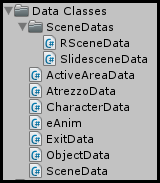
\includegraphics[height=2.5in]{figures/it1/dataclasses.png}
	\caption[Clases de Datos - Prototipo 1]{Vista de carpeta de las clases de datos implementadas en la primera iteración.}
	\label{dataclassesit1}
\end{figure}

Estas clases se auto-generan analizando un \textit{XmlElement} que reciben en su constructor, y por lo general no aportan funcionalidad, salvo excepciones como la función \textit{Check()} que implementan la mayor parte de recursos para verificar si se cumplen todas las condiciones para que dicho recurso pueda ser utilizado.

La mayor parte de clases de datos contienen:
\begin{itemize}
	\item Una serie de Recursos: con soporte de videos y animaciones (implementadas con la clase eAnim y eFrame). Algunas clases implementan su propia clase para manejar sus recursos con Condiciones, como CharacterData con su CharacterResource, o SceneData con su SceneResource, aunque muchas otras simplemente utilizan diccionarios de tipo Dictionary<string,Texture2DHolder> Resources.
	
	\item También tienen una serie de condiciones ante las que decidiran representarese o no, estas condiciones son gestionadas mediante la clase Condition.
	
	\item Algunas clases de datos, además de Recursos y Condiciones, también tienen Efectos que se realizan al interactuar con ellas, o un listado de Acciones que se muestra como un menú contextual al interactuar con ellas.
\end{itemize}

